
\pdfminorversion=4 % for acroread
\documentclass[aspectratio=169,t,xcolor={usenames,dvipsnames}]{beamer}
%\documentclass[t,handout,xcolor={usenames,dvipsnames}]{beamer}
\usepackage{../beamerstyle}
\usepackage{dsfont}
\usepackage{bm}
\usepackage[english]{babel}
\usepackage[utf8]{inputenc}
\usepackage{graphicx}
\usepackage{algorithm}
\usepackage[ruled,vlined,algo2e,linesnumbered]{algorithm2e}
%\usepackage[boxed,vlined]{algorithm2e}
\usepackage{hyperref}
\usepackage{booktabs}
\usepackage{mathtools}

\usepackage{amsmath,amssymb}
\usepackage{listings}
\lstset{frame=lines,framesep=3pt,numbers=left,numberblanklines=false,basicstyle=\ttfamily\small}

\usepackage{subfig}
\usepackage{multicol}
%\usepackage{appendixnumberbeamer}
%
\usepackage{tcolorbox}

\usepackage{pgfplots}
\usepackage{tikz}
\usetikzlibrary{trees} 
\usetikzlibrary{shapes.geometric}
\usetikzlibrary{positioning,shapes,shadows,arrows,calc,mindmap}
\usetikzlibrary{positioning,fadings,through}
\usetikzlibrary{decorations.pathreplacing}
\usetikzlibrary{intersections}
\usetikzlibrary{positioning,fit,calc,shadows,backgrounds}
\pgfdeclarelayer{background}
\pgfdeclarelayer{foreground}
\pgfsetlayers{background,main,foreground}
\tikzstyle{activity}=[rectangle, draw=black, rounded corners, text centered, text width=8em]
\tikzstyle{data}=[rectangle, draw=black, text centered, text width=8em]
\tikzstyle{myarrow}=[->, thick, draw=black]

% Define the layers to draw the diagram
\pgfdeclarelayer{background}
\pgfdeclarelayer{foreground}
\pgfsetlayers{background,main,foreground}

%\usepackage{listings}
%\lstset{numbers=left,
%  showstringspaces=false,
%  frame={tb},
%  captionpos=b,
%  lineskip=0pt,
%  basicstyle=\ttfamily,
%%  extendedchars=true,
%  stepnumber=1,
%  numberstyle=\small,
%  xleftmargin=1em,
%  breaklines
%}

 
\definecolor{blue}{RGB}{0, 74, 153}

\usetheme{Boadilla}
%\useinnertheme{rectangles}
\usecolortheme{whale}
\setbeamercolor{alerted text}{fg=blue}
\useoutertheme{infolines}
\setbeamertemplate{navigation symbols}{\vspace{-5pt}} % to lower the logo
\setbeamercolor{date in head/foot}{bg=blue} % blue
\setbeamercolor{date in head/foot}{fg=white}
\setbeamercolor{author in head/foot}{bg=blue} %blue
\setbeamercolor{title in head/foot}{bg=blue} % blue
\setbeamercolor{title}{fg=white, bg=blue}
\setbeamercolor{block title}{fg=white,bg=blue}
\setbeamercolor{block body}{bg=blue!10}
\setbeamercolor{frametitle}{fg=white, bg=blue}
\setbeamercovered{invisible}

\makeatletter
\setbeamertemplate{footline}
{
  \leavevmode%
  \hbox{%
  \begin{beamercolorbox}[wd=.333333\paperwidth,ht=2.25ex,dp=1ex,center]{author in head/foot}%
    \usebeamerfont{author in head/foot}\insertshortauthor
  \end{beamercolorbox}%
  \begin{beamercolorbox}[wd=.333333\paperwidth,ht=2.25ex,dp=1ex,center]{title in head/foot}%
    \usebeamerfont{title in head/foot}\insertshorttitle
  \end{beamercolorbox}%
  \begin{beamercolorbox}[wd=.333333\paperwidth,ht=2.25ex,dp=1ex,right]{date in head/foot}%
    \usebeamerfont{date in head/foot}Week \@week, Topic \@topicnumber, Slide \insertframenumber{}\hspace*{2em}
%    \insertframenumber\hspace*{2ex} 
  \end{beamercolorbox}}%
  \vskip0pt%
}

\newcommand{\@week}{0}
\newcommand{\@topicnumber}{0}
\newcommand{\week}[1]{\renewcommand{\@week}{#1}}
\newcommand{\topicnumber}[1]{\renewcommand{\@topicnumber}{#1}}

\makeatother

%\pgfdeclareimage[height=1.2cm]{automl}{images/logos/automl.png}
%\pgfdeclareimage[height=1.2cm]{freiburg}{images/logos/freiburg}

%\logo{\pgfuseimage{freiburg}}

\input{../latex_main/macros}





\title[AutoML: Overview]{AutoML: Algorithm Selection} % week title
\subtitle{Performance Models} % video title
\author[Lars Kotthoff]{Bernd Bischl \and Frank Hutter \and \underline{Lars Kotthoff}\newline \and Marius Lindauer \and Joaquin Vanschoren}
\institute{}
\date{}
\week{3}
\topicnumber{4}

% \AtBeginSection[] % Do nothing for \section*
% {
%   \begin{frame}{Outline}
%     \bigskip
%     \vfill
%     \tableofcontents[currentsection]
%   \end{frame}
% }

\begin{document}
	
	\maketitle
	
\begin{frame}[c]{Algorithm Selection}
\begin{center}
\resizebox{.7\textwidth}{!}{%
\tikzset{>=latex}
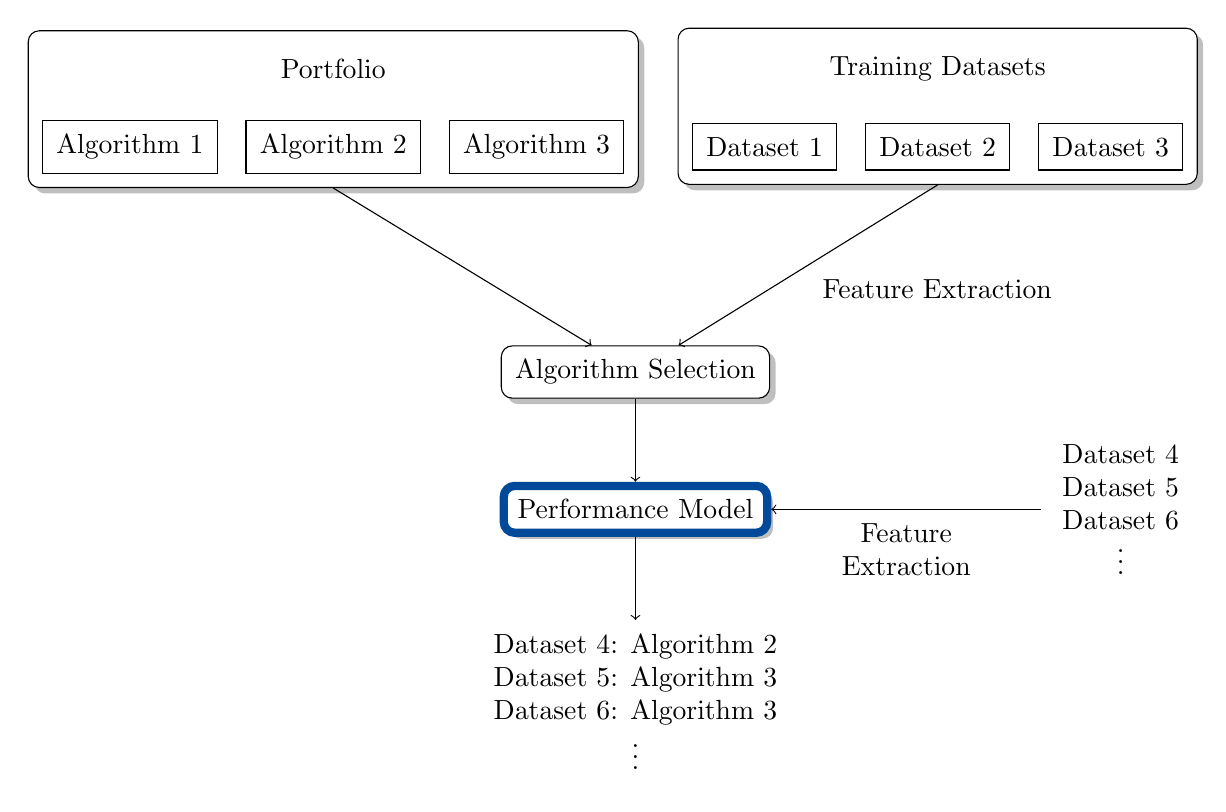
\begin{tikzpicture}[node distance=1em,inner sep=.5em,n/.style={drop
shadow,fill=white,rounded corners},scale=.5]
\node (p) [align=left] {Portfolio};
\node (a2) [rectangle,align=center,below=of p,draw] {Algorithm 2};
\node (a1) [rectangle,align=center,left=of a2,draw] {Algorithm 1};
\node (a3) [rectangle,align=center,right=of a2,draw] {Algorithm 3};
\begin{pgfonlayer}{background}
\node (pc) [n,fit={(p) (a1) (a2) (a3)},draw] {};
\end{pgfonlayer}

\node (i) [align=left,right=15em of p.east] {Training Datasets};
\node (i2) [rectangle,align=center,below=of i,draw] {Dataset 2};
\node (i1) [rectangle,align=center,left=of i2,draw] {Dataset 1};
\node (i3) [rectangle,align=center,right=of i2,draw] {Dataset 3};
\begin{pgfonlayer}{background}
\node (ic) [n,fit={(i) (i1) (i2) (i3)},draw] {};
\end{pgfonlayer}

\node (as) [n,draw,align=left,below=10em of $(p)!0.5!(i)$] {Algorithm Selection};
\node (m) [n,align=left,below=3em of as, rectangle, draw = blue, line width = 3pt] {Performance Model};

\node (it) [align=center,right=10em of m] {Dataset 4\\Dataset 5\\Dataset 6\\$\vdots$};

\node (s) [align=center,below=3em of m] {Dataset 4: Algorithm 2\\Dataset 5: Algorithm 3\\Dataset 6: Algorithm 3\\$\vdots$};

\path [->] (pc.south) edge (as);
\path [->] (ic.south) edge node [below right] {Feature Extraction} (as);
\path [->] ([xshift=-.5em]it.west) edge node [below,align=center] {Feature\\Extraction} (m.east);
\path [->] (as.south) edge (m.north);
\path [->] (m.south) edge (s.north);
\end{tikzpicture}}
\end{center}
\end{frame}

\begin{frame}[c]{Types of Performance Models}
\begin{itemize}
\item models for entire portfolios
\item models for individual algorithms
\item models that are somewhere in between (e.g.\ pairs of algorithms)
\end{itemize}
$\rightarrow$ for each of these, many different machine learning approaches are
suitable
\end{frame}

\begin{frame}[c]{Models for Entire Portfolios}
\begin{itemize}
    \item predict the best algorithm in the portfolio (e.g.\ classifier to use)
\item alternatively: cluster in meta-feature space and assign best algorithm to
    each cluster
\end{itemize}
optional (but important):
\begin{itemize}
\item attach a ``weight'' during learning (e.g.\ the difference between best
    and worst algorithm) to bias model towards the ``important'' datasets
\item special loss metric
\end{itemize}
\end{frame}

\begin{frame}[c]{Models for Individual Algorithms}
\begin{itemize}
\item predict the performance for each algorithm separately
\item combine the predictions to choose the best one
\item for example: predict accuracy, choose algorithm with highest predicted
    accuracy
\end{itemize}
\end{frame}

\begin{frame}[c]{Hybrid Models}
\begin{itemize}
\item for example: consider pairs of algorithms to take relations between them into account
\item for each pair of algorithms, learn model that predicts which one has
    better performance, or predicts performance difference
\item \ldots{}or collaborative filtering approaches
\end{itemize}
\end{frame}

\begin{frame}[c]{Types of Performance Models}
\begin{center}
\resizebox{!}{.8\textheight}{%
\tikzset{>=latex}
\begin{tikzpicture}[node distance=1em,inner sep=.5em,n/.style={drop shadow,fill=white,rounded corners}
]

\node (pm2c) [n,align=center,draw] {Regression Models\\
\begin{tikzpicture}[scale=0.3]
\draw (0,1) .. controls (1,1) .. (4,0) node [right]{A1};
\draw (0,0) .. controls (1,0) .. (4,4) node [right]{A2};
\draw (0,2) .. controls (2,3) .. (4,2) node [right]{A3};
\end{tikzpicture}
};

\node (pm2cr) [align=left,right=3em of pm2c] {A1: 1.2\\\textbf{A2: 4.5}\\A3: 3.9};

\node (pm1c) [n,align=center,above=of pm2c,draw] {Classification Model\\[1em]
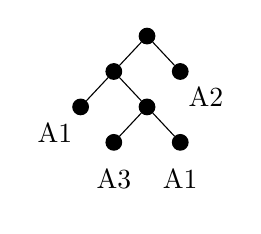
\begin{tikzpicture}[scale=0.3,sibling distance=8em,every node/.style={circle,fill=black,inner sep=.2em}]
\node (pm1) [draw] {}
child{ node [draw] {}
        child{ node [draw,label={below left:A1}] {} }
        child{ node [draw] {}
                        child{ node [draw,label={below:A3}] {}}
                        child{ node [draw,label={below:A1}] {}}
        }
}
child{ node [draw,label={below right:A2}] {} }
;
\end{tikzpicture}
};

\node (pm1cr) [align=left,right=3em of pm1c] {\textbf{A1}};

\node (pm3c) [n,align=center,below=of pm2c,draw] {Pairwise Classification Models\\[1em]
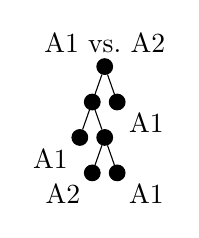
\begin{tikzpicture}[scale=0.3,every label/.append style={shape=rectangle},sibling distance=3em,every node/.style={circle,fill=black,inner sep=.2em}]
\node [draw,label={above:A1 vs.\ A2}] {}
child{ node [draw] {}
        child{ node [draw,label={below left:A1}] {} }
        child{ node [draw] {}
                        child{ node [draw,label={below left:A2}] {}}
                        child{ node [draw,label={below right:A1}] {}}
        }
}
child{ node [draw,label={below right:A1}] {} }
;
\end{tikzpicture}
\hspace{1em}
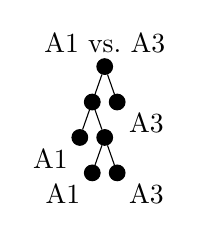
\begin{tikzpicture}[scale=0.3,every label/.append style={shape=rectangle},sibling distance=3em,every node/.style={circle,fill=black,inner sep=.2em}]
\node [draw,label={above:A1 vs.\ A3}] {}
child{ node [draw] {}
        child{ node [draw,label={below left:A1}] {} }
        child{ node [draw] {}
                        child{ node [draw,label={below left:A1}] {}}
                        child{ node [draw,label={below right:A3}] {}}
        }
}
child{ node [draw,label={below right:A3}] {} }
;
\end{tikzpicture}
\hspace{1em}
\raisebox{3.7em}{\ldots}
};

\node (pm3cr) [align=left,right=1em of pm3c] {A1: 1 vote\\A2: 0 votes\\\textbf{A3: 2 votes}};

\node (pm4c) [n,align=center,below=of pm3c,draw] {Pairwise Regression Models\\[1em]
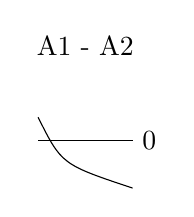
\begin{tikzpicture}[scale=0.3]
\draw (2,6) node {A1 - A2};
\draw (0,3) .. controls (1,1) .. (4,0);
\draw (0,2) -- (4,2) node [right] {0};
\end{tikzpicture}
\hspace{1em}
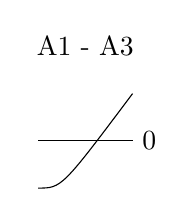
\begin{tikzpicture}[scale=0.3]
\draw (2,6) node {A1 - A3};
\draw (0,0) .. controls (1,0) .. (4,4);
\draw (0,2) -- (4,2) node [right] {0};
\end{tikzpicture}
\hspace{1em}
\raisebox{2em}{\ldots}
};

\node (pm4cr) [align=left,right=1em of pm4c] {A1: -1.3\\A2: 0.4\\\textbf{A3: 1.7}};

\node (pmc) [fit={(pm1c) (pm1cr) (pm2c) (pm2cr) (pm3c) (pm3cr) (pm4c) (pm4cr)},draw,dashed] {};

\node (it) [align=center,left=3em of pmc] {Dataset 1\\Dataset 2\\Dataset 3\\$\vdots$};

\node (ps) [align=center,right=3em of pmc] {Dataset 1: Algorithm 2\\Dataset 2:
Algorithm 1\\Dataset 3: Algorithm 3\\$\vdots$};

\path [->] (it) edge (pmc);
\path [->] (pmc) edge (ps);
\path [->] (pm1c) edge (pm1cr);
\path [->] (pm2c) edge (pm2cr);
\path [->] (pm3c) edge (pm3cr);
\end{tikzpicture}}
\end{center}
\end{frame}

\begin{frame}[c]{Types of Predictions/Algorithm Selectors}
\begin{itemize}
\item best algorithm (and its performance)
\item $n$ best algorithms ranked
\item ensemble of $n$ best algorithms
\end{itemize}
\end{frame}

\begin{frame}[c]{Time/Frequency of Prediction}
\begin{itemize}
\item one-shot
    \begin{itemize}
    \item select algorithm(s) once
    \item want to process single dataset and choose the best approach
    \end{itemize}
\item multi-shot
    \begin{itemize}
    \item continuously monitor dataset(s) features and/or performance
    \item for example on data streams or to process sets of datasets
    \end{itemize}
\end{itemize}
\end{frame}

\end{document}
